\subsection{FT Properties}
\begin{definition}
    We denote the Fourier Transform pair as:
    \[
    x(t) \overset{F}{\leftrightarrow} X(f)
    \]
    \vspace{1em}

    \textbf{Fourier Transform:}
    \[
    X(f) = \int_{-\infty}^{\infty} x(t) e^{-j 2 \pi f t} \, dt
    \]
    \[
    x(t) = \int_{-\infty}^{\infty} X(f) e^{j 2 \pi f t} \, df
    \]
    \vspace{1em}

    \textbf{Fourier Transform Conventions}
    \begin{itemize}
        \item Use lowercase letters for time domain functions (e.g., \( x(t) \)).
        \item Use uppercase letters for frequency domain functions (e.g., \( X(f) \)).
    \end{itemize}
\end{definition}

\subsubsection{Common Fourier Transform Pairs}
\begin{definition}
    \begin{enumerate}
    \item For the rectangular function:
    \[
    \text{rect}(t) \overset{F}{\leftrightarrow} \text{sinc}(f)
    \]
    \customFigure[0.75]{00_Images/RECT3.png}{Time domain to frequency domain.}

    \item For \( x(t) = e^{-at} u(t) \):
    \begin{equation*}
        e^{-at} u(t) \overset{F}{\leftrightarrow} \frac{1}{a + j 2 \pi f} \text{ for $a > 0$}
    \end{equation*}
    \begin{itemize}
        \item \textbf{Proof:} \begin{align*}
            X(f) &= \int_{0}^{\infty} e^{-at} e^{-j 2 \pi f t} \, dt \\
                &= \left. \frac{e^{-(a + j 2 \pi f)t}}{-(a + j 2 \pi f)} \right|_0^{\infty} = \frac{1}{a + j 2 \pi f} \quad \text{for } a > 0
        \end{align*}
    \end{itemize}

    \item For \( x(t) = \delta(t) \):
    \begin{equation*}
        \delta(t) \overset{F}{\leftrightarrow} 1 
    \end{equation*}
    \begin{itemize}
        \item \textbf{Proof:} $X(f) = \int_{-\infty}^{\infty} \delta(t) e^{-j 2 \pi f t} \, dt =  \int_{-\infty}^{\infty} \delta(t) e^{j0} \, dt = 1$
    \end{itemize}

    \item For \( X(f) = \delta(f) \):
    \begin{equation*}
        1 \overset{F}{\leftrightarrow} \delta(f)
    \end{equation*}
    \begin{itemize}
        \item \textbf{Proof:} $x(t) = \int_{-\infty}^{\infty} \delta(f) e^{j 2 \pi f t} \, df = \int_{-\infty}^{\infty} \delta(f) e^{j 0} \, df = 1$
    \end{itemize}

    \item For \( x(t) = \delta(t - t_0) \):
    \begin{equation*}
        \delta(t - t_0) \overset{F}{\leftrightarrow} e^{-j 2 \pi f t_0} 
    \end{equation*}
    \begin{itemize}
        \item \textbf{Proof:} $X(f) = \int_{-\infty}^{\infty} \delta(t - t_0) e^{-j 2 \pi f t} \, dt = e^{-j 2 \pi f t_0}$
    \end{itemize}
    \customFigure[0.5]{00_Images/P1.png}{.}

    \item For \( X(f) = \delta(f - f_0) \):
    \begin{equation*}
        e^{j 2 \pi f_0 t} \overset{F}{\leftrightarrow} \delta(f - f_0)
    \end{equation*}
    \begin{itemize}
        \item \textbf{Proof:} $x(t) = \int_{-\infty}^{\infty} \delta(f - f_0) e^{j 2 \pi f t} \, df = e^{j 2 \pi f_0 t}$
    \end{itemize}
    \customFigure[0.5]{00_Images/P2.png}{.}

    \item \textbf{Linearity property:} If \( x \overset{F}{\leftrightarrow} X \) and \( y \overset{F}{\leftrightarrow} Y \), then
    \[
    \alpha x + \beta y \overset{F}{\leftrightarrow} \alpha X + \beta Y \quad \text{for all } \alpha, \beta \in \mathbb{C}
    \]
    \begin{itemize}
        \item \textbf{Proof:}
        \begin{align*}
            \int_{-\infty}^{\infty} \left( \alpha x(t) + \beta y(t) \right) e^{-j 2 \pi f t} \, dt &= \alpha \int_{-\infty}^{\infty} x(t) e^{-j 2 \pi f t} \, dt + \beta \int_{-\infty}^{\infty} y(t) e^{-j 2 \pi f t} \, dt \\
            &= \alpha X + \beta Y
        \end{align*}
    \end{itemize}
    \item \textbf{General linearity property:} 
    \[
    \sum_{k \in \mathbb{Z}} \alpha_k x_k \overset{F}{\leftrightarrow} \sum_{k \in \mathbb{Z}} \alpha_k X_k
    \]
    \end{enumerate}
\end{definition}

\subsection{Fourier Series Transforms of Periodic Signals (4.2)}
\begin{definition}
    Suppose \( x \underset{T}{\overset{FS}{\leftrightarrow}} c_k \), then
    \[
    x(t) = \sum_{k \in \mathbb{Z}} c_k e^{j 2 \pi \frac{k}{T} t} \rightarrow X(f) = \sum_{k \in \mathbb{Z}} c_k \delta\left(f - \frac{k}{T}\right) \quad \text{(Line Spectrum)}
    \]
    \begin{itemize}
        \item i.e. Periodic signals have a line spectrum as the Fourier Transform.
    \end{itemize}
\end{definition}

\begin{example}
    \begin{enumerate}
        \item For \( x(t) = \cos(2 \pi f_0 t) \):
           \begin{align*}
               x(t) &= \frac{1}{2} e^{j 2 \pi f_0 t} + \frac{1}{2} e^{-j 2 \pi f_0 t} \\
               X(f) &= \frac{1}{2} \delta(f - f_0) + \frac{1}{2} \delta(f + f_0)
           \end{align*}
           \customFigure[0.5]{00_Images/COS.png}{.}
        
        \item For \( y(t) = \sin(2 \pi f_0 t) \):
           \begin{align*}
               y(t) &= \frac{1}{2j} e^{j 2 \pi f_0 t} - \frac{1}{2j} e^{-j 2 \pi f_0 t} \\
               X(f) &= \frac{1}{2j} \delta(f - f_0) - \frac{1}{2j} \delta(f + f_0)
           \end{align*}
           \customFigure[0.5]{00_Images/SINE.png}{.}
        
        \item For the periodic rectangle function.
        \[
        x(t) \underset{T}{\overset{FS}{\longleftrightarrow}} c_k = \frac{1}{T} \, \text{sinc} \left( \frac{k}{T} \right)
        \]
        \customFigure[0.5]{00_Images/RECT4.png}{.}
        \[
        X(f) = \sum_{k \in \mathbb{Z}} \frac{1}{T} \, \text{sinc} \left( \frac{k}{T} \right) \delta \left( f - \frac{k}{T} \right)
        \]
        \customFigure[0.5]{00_Images/REC5.png}{Also a line spectrum (note, in reality these lines diverge to infinity, but we have just drawn in this manner to scale the area to $1$)}

        \item For the rectangular pulse train:
           \[
           x(t) = \sum_{k \in \mathbb{Z}} \delta(t - kT) \underset{T}{\overset{FS}{\longleftrightarrow}} c_k = \frac{1}{T}
           \]
           \[
           X(f) = \sum_{k \in \mathbb{Z}} \frac{1}{T} \delta\left(f - \frac{k}{T}\right)
           \]
           This represents a \textbf{picket fence function}, which will be significant in sampling theory.
           \customFigure[0.75]{00_Images/PF.png}{Picket fence.}
           \begin{itemize}
            \item \textbf{Reciprocal Spacing:} If the spacing is wide in the time domain, then the spacing will be narrow in the frequency domain. Vice versa.
           \end{itemize}
    \end{enumerate}
\end{example}

\subsection{Properties of Fourier Transform (MIDTERM CUTOFF EXCLUSIVE)}
\begin{warning}
    \begin{itemize}
        \item Time domain is on left side of FT Pair and frequency domain is on the right side.
    \end{itemize}
\end{warning}

\subsubsection{1. Linearity}
\begin{definition}
    If \( x(t) \overset{\mathcal{F}}{\leftrightarrow} X(f) \) and \( y(t) \overset{\mathcal{F}}{\leftrightarrow} Y(f) \), then
\[
\alpha x(t) + \beta y(t) \overset{\mathcal{F}}{\leftrightarrow} \alpha X(f) + \beta Y(f), \quad \forall \, \alpha, \beta \in \mathbb{C}.
\]
\end{definition}

\subsubsection{2. Time-shifting}
\begin{definition}
    If \( x(t) \overset{\mathcal{F}}{\leftrightarrow} X(f) \), then
\[
x(t - t_0) \overset{\mathcal{F}}{\leftrightarrow} e^{-j 2 \pi f t_0} X(f).
\]
\end{definition}

\begin{derivation}
    \textbf{Proof:}
    \begin{align*}
    \mathcal{F}^{-1} \left( e^{-j 2 \pi f t_0} X(f) \right) &= \int_{-\infty}^{\infty} X(f) e^{-j 2 \pi f t_0} e^{j 2 \pi f t} \, df \\
    &= \int_{-\infty}^{\infty} X(f) e^{j 2 \pi f (t - t_0)} \, df \\
    &= x(t - t_0).
    \end{align*}
\end{derivation}

\subsubsection{3. Frequency-shifting (Modulation)}
\begin{definition}
    If \( x(t) \overset{\mathcal{F}}{\leftrightarrow} X(f) \), then
    \[
    e^{j 2 \pi f_0 t} x(t) \overset{\mathcal{F}}{\leftrightarrow} X(f - f_0).
    \]
\end{definition}

\begin{derivation}
    \textbf{Proof:}
    \begin{align*}
    \mathcal{F} \left( e^{j 2 \pi f_0 t} x(t) \right) &= \int_{-\infty}^{\infty} e^{j 2 \pi f_0 t} x(t) e^{-j 2 \pi f t} \, dt \\
    &= \int_{-\infty}^{\infty} x(t) e^{-j 2 \pi (f - f_0) t} \, dt \\
    &= X(f - f_0).
    \end{align*}
\end{derivation}

\subsubsection{4. Time-reversal}
\begin{definition}
    If \( x(t) \overset{\mathcal{F}}{\leftrightarrow} X(f) \), then
    \[
    \tilde{x}(t) = x(-t) \overset{\mathcal{F}}{\leftrightarrow} \tilde{X}(f) = X(-f).
    \]
\end{definition}

\begin{derivation}
    \textbf{Proof:}
    \begin{align*}
    \mathcal{F} \left( x(-t) \right) &= \int_{-\infty}^{\infty} x(-t) e^{-j 2 \pi f t} \, dt \\
    &= \int_{\infty}^{-\infty} x(s) e^{-j 2 \pi f (-s)} (-ds) \quad \text{(substitute } s = -t, \, ds = -dt) \\
    &= \int_{-\infty}^{\infty} x(s) e^{-j 2 \pi (-f) s} \, ds \\
    &= X(-f) \\
    &= \tilde{X}(f).
    \end{align*}
\end{derivation}

\subsubsection{5. Conjugation}
\begin{definition}
    If \( x(t) \overset{\mathcal{F}}{\leftrightarrow} X(f) \), then
    \[
    x^*(t) \overset{\mathcal{F}}{\leftrightarrow} \tilde{X}^*(f) = X^*(-f).
    \]
\end{definition}

\begin{derivation}
    \textbf{Proof:}
    \begin{align*}
    \mathcal{F} \left( x^*(t) \right) &= \int_{-\infty}^{\infty} x^*(t) e^{-j 2 \pi f t} \, dt \\
    &= \left( \int_{-\infty}^{\infty} x(t) e^{j 2 \pi f t} \, dt \right)^* \\
    &= \left( \int_{-\infty}^{\infty} x(t) e^{-j 2 \pi (-f) t} \, dt \right)^* \\
    &= \left( X(-f) \right)^* \\
    &= X^*(-f).
    \end{align*}
\end{derivation}

\subsubsection{6. Duality}
\begin{definition}
    If \( x(t) \overset{\mathcal{F}}{\leftrightarrow} X(f) \), then
    \[
    X(t) \overset{\mathcal{F}}{\leftrightarrow} \tilde{x}(f) = x(-f).
    \]
\end{definition}

\begin{derivation}
    \textbf{Proof:}
    \begin{align*}
    X(f) &= \int_{-\infty}^{\infty} x(t) e^{-j 2 \pi f t} \, dt, \\
    X(t) &= \int_{-\infty}^{\infty} x(s) e^{-j 2 \pi t s} \, ds, \quad (t \rightarrow s) \text{ and } (f \rightarrow t) \\
    \mathcal{F}(X(t)) &= \int_{-\infty}^{\infty} X(t) e^{-j 2 \pi f t} \, dt \\
    &= \int_{-\infty}^{\infty} \left( \int_{-\infty}^{\infty} x(s) e^{-j 2 \pi t s} \, ds \right) e^{-j 2 \pi f t} \, dt \\
    &= \int_{-\infty}^{\infty} x(s) \int_{-\infty}^{\infty} e^{-j 2 \pi t s}  e^{-j 2 \pi f t} \, dt \, ds \\
    &= \int_{-\infty}^{\infty} x(s) \delta(s + f) \, ds \\
    &= x(-f) \\
    &= \tilde{x}(f)
    \end{align*}
\end{derivation}

\begin{definition}
    \begin{center}
        \begin{tikzpicture}
            % Nodes
            \node (X) at (0, 2) {\( x \)};
            \node (XF) at (2, 2) {\( X \)};
            \node (XTildeF) at (2, 0) {\( \tilde{x} \)};
            \node (XTilde) at (0, 0) {\( \tilde{X} \)};
    
            % Arrows
            \draw[->] (X) -- node[above] {\( \mathcal{F} \)} (XF);
            \draw[<-] (XTilde) -- node[below] {\( \mathcal{F} \)} (XTildeF);
            \draw[<-] (X) -- node[left] {\( \mathcal{F} \)} (XTilde);
            \draw[->] (XF) -- node[right] {\( \mathcal{F} \)} (XTildeF);
        \end{tikzpicture}
    \end{center}

    \begin{center}
        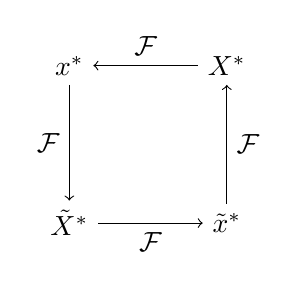
\begin{tikzpicture}
            % Nodes
            \node (XStar) at (0, 2) {\( x^* \)};
            \node (XFStar) at (2, 2) {\( X^* \)};
            \node (XTildeFStar) at (2, 0) {\( \tilde{x}^* \)};
            \node (XTildeStar) at (0, 0) {\( \tilde{X}^* \)};
    
            % Arrows
            \draw[<-] (XStar) -- node[above] {\( \mathcal{F} \)} (XFStar);
            \draw[->] (XTildeStar) -- node[below] {\( \mathcal{F} \)} (XTildeFStar);
            \draw[->] (XStar) -- node[left] {\( \mathcal{F} \)} (XTildeStar);
            \draw[<-] (XFStar) -- node[right] {\( \mathcal{F} \)} (XTildeFStar);
        \end{tikzpicture}
    \end{center}
    \begin{itemize}
        \item \textbf{Note:} These are all in the time domain bc we are applying the Fourier Transform.
    \end{itemize}
\end{definition}

\begin{example}
    \customFigure[0.75]{00_Images/DU.png}{Duality example}
\end{example}

\subsection{Time Scaling Property}
\begin{definition}
    If \( x \overset{\mathcal{F}}{\leftrightarrow} X \), then:
    \begin{align*}
    x(at) &\overset{\mathcal{F}}{\leftrightarrow} \frac{1}{|a|} X\left( \frac{f}{a} \right) \\
    |a| x(at) &\overset{\mathcal{F}}{\leftrightarrow} X\left( \frac{f}{a} \right) 
    \end{align*}
    for $a \in \mathbb{R}$, $a \neq 0$.
    \begin{itemize}
        \item \textbf{Note:} Time stretching is frequency inversie stretching. 
    \end{itemize}
\end{definition}

\begin{derivation}
    \textbf{Proof:}
    If $a>0$
    \begin{align*}
        \mathcal{F}\{x(at)\} &= \int_{-\infty}^{\infty} x(at) e^{-j 2 \pi f t} \, dt \\
        &= \int_{-\infty}^{\infty} x(s) e^{-j 2 \pi \frac{f}{a} s} \frac{ds}{a} \quad \text{(substitute } s = at, \, ds = a \, dt\text{)} \\
        &= \frac{1}{a} X\left(\frac{f}{a}\right)
    \end{align*}
    
    If $a<0$
    \begin{align*}
        \mathcal{F}\{x(at)\} &= \int_{-\infty}^{\infty} x(at) e^{-j 2 \pi f t} \, dt \\
        &= \int_{-\infty}^{\infty} x(s) e^{-j 2 \pi \frac{f}{a} s} \frac{ds}{a} \quad \text{(substitute } s = at, \, ds = a \, dt\text{)} \\
        \mathcal{F}\{x(at)\} &= -\frac{1}{a} X\left(\frac{f}{a}\right)
    \end{align*}
\end{derivation}

\begin{example}
    \begin{align*}
        \text{rect}(t) &\leftrightarrow \text{sinc}(f) \\
        \text{rect}\left(\frac{t}{T}\right) &\leftrightarrow T \, \text{sinc}(f T)
    \end{align*}

    \customFigure[0.5]{00_Images/C1.png}{Rect vs. Sinc}
    \begin{center}
        \begin{multicols}{2}
            \textbf{Time Domain}
            \begin{itemize}
                \item Narrow in time $(T \text{ small})$: "fast"
                \item Wide in time $(T \text{ large})$: "slow"
            \end{itemize}
    
            \columnbreak
    
            \textbf{Frequency Domain}
            \begin{itemize}
                \item Wide in frequency $\left(\frac{1}{T} \text{ large}\right)$: "wideband"
                \item Narrow in frequency $\left(\frac{1}{T} \text{ small}\right)$: "narrowband"
            \end{itemize}
        \end{multicols}
    \end{center}
\end{example}

\subsection{Unitarity (Calculate Energy Easily)}

\begin{definition}
    Recall that the inner product of two functions \( x(t) \) and \( y(t) \) over \( (-\infty, \infty) \) is defined as:
    \begin{align*}
    \langle x, y \rangle &= \int_{-\infty}^{\infty} x(t) y^*(t) \, dt.
    \end{align*}

    For a function \( x(t) \), its energy is given by:
    \begin{align*}
    \langle x, x \rangle &= \int_{-\infty}^{\infty} |x(t)|^2 \, dt = E_x.
    \end{align*}
\end{definition}

\begin{definition}
    If \( x \overset{\mathcal{F}}{\leftrightarrow} X \) and \( y \overset{\mathcal{F}}{\leftrightarrow} Y \), then 
    \begin{align*}
        \langle x, y \rangle = \langle X, Y \rangle &= \int_{-\infty}^{\infty} X(f) Y^*(f) \, df.
    \end{align*}
\end{definition}

\begin{derivation}
    \textbf{Proof:}
    \begin{align*}
    \langle x, y \rangle &= \int_{-\infty}^{\infty} x(t) y^*(t) \, dt \\
    &= \int_{-\infty}^{\infty} \left( \int_{-\infty}^{\infty} X(f_1) e^{j 2 \pi f_1 t} \, df_1 \right) \left( \int_{-\infty}^{\infty} Y(f_2) e^{j 2 \pi f_2 t} \, df_2 \right)^* \, dt \\
    &= \int_{-\infty}^{\infty} \int_{-\infty}^{\infty} X(f_1) Y^*(f_2) \left( \int_{-\infty}^{\infty} e^{j 2 \pi (f_1 - f_2) t} \, dt \right) df_1 \, df_2 \\
    &= \int_{-\infty}^{\infty} \int_{-\infty}^{\infty} X(f_1) Y^*(f_2) \delta(f_1 - f_2) \, df_1 \, df_2 \quad \text{due to FT pair}\\
    &= \int_{-\infty}^{\infty} X(f) Y^*(f) \, df \quad \text{due to sifting property}\\
    &= \langle X, Y \rangle.
    \end{align*}
\end{derivation}

\subsection{Parseval's Relation}
\begin{definition}
    If \( x \overset{\mathcal{F}}{\leftrightarrow} X \) then
    \[
    \int_{-\infty}^{\infty} |x(t)|^2 \, dt = \int_{-\infty}^{\infty} |X(f)|^2 \, df
    \]
\end{definition}

\begin{derivation}
    \textbf{Proof:}
    \[
    \int_{-\infty}^{\infty} |x(t)|^2 \, dt = \langle x, x \rangle = \langle X, X \rangle = \int_{-\infty}^{\infty} |X(f)|^2 \, df \quad \text{by unitarity}
    \]
\end{derivation}

\begin{example}
    \textbf{Example:}
    Let \( x(t) = \operatorname{sinc}(t) \).
    \begin{align*}
        E_x &= \int_{-\infty}^{\infty} \operatorname{sinc}^2(t) \, dt \\ 
        &= \int_{-\infty}^{\infty} \frac{\sin^2(\pi t)}{(\pi t)^2} \, dt \\
        &= \int_{-\infty}^{\infty} \operatorname{rect}^2(f) \, df \\
        &= 1
    \end{align*}
\end{example}

\subsection{Differentiation Property}
\begin{definition}
    If \( x \overset{\mathcal{F}}{\leftrightarrow} X \), then:
    \begin{align*}
    \frac{d}{dt} x(t) \overset{\mathcal{F}}{\leftrightarrow} j2\pi f X(f).
    \end{align*}
\end{definition}

\begin{derivation}
    \textbf{Proof:}
    \begin{align*}
    x(t) &= \int_{-\infty}^{\infty} X(f) e^{j 2 \pi f t} \, df, \\
    \frac{d}{dt} x(t) &= \int_{-\infty}^{\infty} X(f) \left( j 2 \pi f \right) e^{j 2 \pi f t} \, df, \\
    &= \mathcal{F}^{-1} \left( j 2 \pi f X(f) \right).
    \end{align*}
\end{derivation}

\begin{warning}
    Choose the domain that is most convienent for the problem.
\end{warning}

\subsection{Convolution Property}
\begin{definition}
    \begin{itemize}
        \item If \( x(t) \overset{\mathcal{F}}{\leftrightarrow} X(f) \) and \( y(t) \overset{\mathcal{F}}{\leftrightarrow} Y(f) \), then
        \[
        x(t) * y(t) \overset{\mathcal{F}}{\leftrightarrow} X(f) Y(f).
        \]
        \item Convolution in the time domain becomes multiplication in the frequency domain.
        \item This justifies the use of the frequency domain for certain computations.
    \end{itemize}
\end{definition}

\begin{derivation}
    \textbf{Proof:}
    \begin{align*}
        \mathcal{F}\{x * y\} &= \int_{-\infty}^{\infty} (x * y)(t) e^{-j 2 \pi f t} \, dt \\
        &= \int_{-\infty}^{\infty} \int_{-\infty}^{\infty} x(\tau) y(t - \tau) \, d\tau \, e^{-j 2 \pi f t} \, dt \\
        &= \int_{-\infty}^{\infty} x(\tau) \int_{-\infty}^{\infty} y(t - \tau) e^{-j 2 \pi f t} \, dt \, d\tau \\
        &= \int_{-\infty}^{\infty} x(\tau) \left( \int_{-\infty}^{\infty} y(t - \tau) e^{-j 2 \pi f t} \, dt \right) d\tau \\
        &= \int_{-\infty}^{\infty} x(\tau) \left( Y(f) e^{-j 2 \pi f \tau} \right) d\tau \\
        &= \left( \int_{-\infty}^{\infty} x(\tau) e^{-j 2 \pi f \tau} d\tau \right) Y(f) \\
        &= X(f) Y(f).
    \end{align*}
\end{derivation}

\subsubsection{Cascading Systems:}
\begin{definition}
    \customFigure[0.75]{00_Images/H1.png}{Cascading Systems}
\end{definition}

\begin{example}
    \customFigure[0.75]{00_Images/H2.png}{Cascading Systems}
    \customFigure[0.75]{00_Images/H.png}{Cascading Systems}
\end{example}

\subsubsection{Non-Ideal Low Pass Filter}
\begin{example}
    \customFigure[0.75]{00_Images/H4.png}{Cascading Systems}
\end{example}

\subsection{Sign Function}
\begin{definition}
    \[
\text{sgn}(t) = 
\begin{cases}
    1, & t > 0 \\
    0, & t = 0 \\
    -1, & t < 0
\end{cases}
\]
    \customFigure[0.75]{00_Images/SGN.png}{Sign function}
\end{definition}

\begin{definition}
    \begin{equation*}
        \text{sgn}(t) \overset{\mathcal{F}}{\leftrightarrow} \frac{1}{j \pi f}.
    \end{equation*}
\end{definition}

\begin{definition}
    \begin{equation*}
        u(t) \overset{\mathcal{F}}{\leftrightarrow} \frac{1}{2} \delta(f) + \frac{1}{j 2 \pi f}.
    \end{equation*}
\end{definition}

\begin{derivation}
    \textbf{Proof:}
\[
x_\alpha(t) =
\begin{cases}
    e^{-\alpha t}, & \text{if } t > 0, \\
    0, & \text{if } t = 0, \\
    -e^{-\alpha t}, & \text{if } t < 0,
\end{cases}
\]
where \( \alpha > 0 \).

\customFigure[0.75]{00_Images/S.png}{Sign function}
\bigskip

\textbf{Limit as } \( \alpha \to 0 \):
\[
\lim_{\alpha \to 0} x_\alpha(t) = \text{sgn}(t).
\]



\begin{align*}
    X_\alpha(f) &= \int_{-\infty}^{\infty} x_\alpha(t) e^{-j 2 \pi f t} \, dt \\
    &= \int_{-\infty}^{0} -e^{-\alpha t} e^{-j 2 \pi f t} \, dt + \int_{0}^{\infty} e^{-\alpha t} e^{-j 2 \pi f t} \, dt \\
    &= -\frac{1}{\alpha - j 2 \pi f} + \frac{1}{\alpha + j 2 \pi f} \\
    &= \frac{4 \pi f}{j (\alpha^2 + 4 \pi^2 f^2)}.
\end{align*}

\textbf{As \( \alpha \to 0 \):}
\begin{align*}
    x_\alpha(f) &\to \lim_{\alpha \to 0} \frac{4 \pi f}{j (\alpha^2 + 4 \pi^2 f^2)} \\
    &= \frac{4 \pi f}{j \cdot 4 \pi^2 f^2} = \frac{1}{j \pi f}.
\end{align*}

\textbf{Therefore:}
\[
\text{sgn}(t) \overset{\mathcal{F}}{\leftrightarrow} \frac{1}{j \pi f}.
\]

\bigskip

\textbf{Note that:}
\[
u(t) = \frac{1}{2} \left(1 + \text{sgn}(t)\right).
\]

\[
u(t) \overset{\mathcal{F}}{\leftrightarrow} \frac{1}{2} \delta(f) + \frac{1}{j 2 \pi f}.
\]
\end{derivation}

\subsubsection{Recovering Unit Impulse from Unit Step}
\begin{derivation}
    Since $\frac{d}{dt} u(t) = \delta(t)$, then
    \begin{align*}
        \frac{d}{dt} u(t) = \delta(t) &\overset{\mathcal{F}}{\leftrightarrow} j2\pi f \left( \frac{1}{j2\pi f} + \frac{1}{2} \delta(f) \right) = 1 + j\pi f \delta(f) = 1
    \end{align*}        
    \begin{itemize}
        \item \textbf{Note:} Last term goes to $0$ since $j\pi f$ is $0$ at $f=0$ (i.e. where the delta function is).
    \end{itemize}
\end{derivation}

\subsection{Integration Property}
\begin{definition}
    $\text{If } x(t) \overset{\mathcal{F}}{\leftrightarrow} X(f),$
\begin{equation*}
\int_{-\infty}^{t} x(\tau) d\tau \overset{\mathcal{F}}{\leftrightarrow} \frac{1}{j2\pi f} X(f) + \frac{1}{2} X(0) \delta(f)
\end{equation*}
\end{definition}

\begin{derivation}
    Since $\int_{-\infty}^{t} x(\tau) d\tau = x(t) * u(t)$
    \begin{align*}
        x(t) * u(t) \overset{\mathcal{F}}{\leftrightarrow} &X(f) U(f) \\
        &= X(f) \left( \frac{1}{j2\pi f} + \frac{1}{2} \delta(f) \right) \\
        &= \frac{X(f)}{j2\pi f} + \frac{1}{2} X(f) \delta(f)
        \end{align*}        
\end{derivation}

\begin{example}
    \customFigure[0.75]{00_Images/SC.png}{Integration Property Example}
\end{example}

\subsection{Multiplication Property}
\begin{definition}
    $ \text{If } x(t) \overset{\mathcal{F}}{\leftrightarrow} X(f), y(t) \overset{\mathcal{F}}{\leftrightarrow} Y(f), \text{ then } x(t) y(t) \overset{\mathcal{F}}{\leftrightarrow} X(f) * Y(f)$
\end{definition}

\begin{derivation}
    \begin{align*}
        \mathcal{F}^{-1} \left( X(f) * Y(f) \right) &= \mathcal{F}^{-1} \left( \int_{-\infty}^{\infty} X(\lambda) Y(f - \lambda) d\lambda \right) \\
        &= \int_{-\infty}^{\infty} \int_{-\infty}^{\infty} X(\lambda) Y(f - \lambda) d\lambda e^{j 2 \pi f t} df \\
        &= \int_{-\infty}^{\infty} X(\lambda) \int_{-\infty}^{\infty} Y(f - \lambda) e^{j2\pi ft} df d\lambda \\
        &\overset{s=f-\lambda}{=} \int_{-\infty}^{\infty} X(\lambda) \int_{-\infty}^{\infty} Y(s) e^{j2\pi (s + \lambda)t} ds d\lambda \\
        &= \int_{-\infty}^{\infty} X(\lambda) e^{j2\pi \lambda t} \left( \int_{-\infty}^{\infty} Y(s) e^{j2\pi st} ds \right) d\lambda \\
        &= x(t) y(t)
        \end{align*}
\end{derivation}
